\documentclass[aspectratio=169]{beamer}
\usepackage[utf8]{inputenc}
\usepackage[T1]{fontenc}
\usepackage{booktabs}
\usepackage{colortbl}
\usepackage{graphicx}
\usepackage{xcolor}
\usepackage{tikz}
\usetikzlibrary{positioning}
\usepackage{pgfplots}
\pgfplotsset{compat=1.18}
\usepackage{amsmath}
\usepackage{tcolorbox}
\tcbuselibrary{skins}

\definecolor{cdark}{HTML}{0D2137}
\definecolor{cmid}{HTML}{065A82}
\definecolor{cteal}{HTML}{02C39A}
\definecolor{clight}{HTML}{E8F4F8}
\definecolor{ctext}{HTML}{1A2E40}
\definecolor{cmuted}{HTML}{607D8B}
\definecolor{cwarn}{HTML}{F4A261}
\definecolor{cgap}{HTML}{E63946}
\definecolor{caccent}{HTML}{A0BFD0}
\definecolor{cbg2}{HTML}{028090}

\usetheme{default}
\usecolortheme{default}
\setbeamertemplate{navigation symbols}{}
\usefonttheme{professionalfonts}
\setbeamerfont{frametitle}{size=\large,series=\bfseries}
\setbeamercolor{frametitle}{fg=cdark,bg=white}
\setbeamercolor{normal text}{fg=ctext}
\setbeamercolor{background canvas}{bg=white}
\setbeamercolor{item}{fg=cteal}

\addtobeamertemplate{frametitle}{}{%
  \vspace{-4pt}\textcolor{cteal}{\hrule height 1.5pt}\vspace{3pt}}

\setbeamertemplate{footline}{%
  \leavevmode\hbox{%
    \begin{beamercolorbox}[wd=0.65\paperwidth,ht=2.2ex,dp=1ex,leftskip=4pt]{normal text}%
      \tiny\color{cmuted}An Pham \textbar{} LIRMM--ADVANSE \textbar{} Luc \& Reda%
    \end{beamercolorbox}%
    \begin{beamercolorbox}[wd=0.35\paperwidth,ht=2.2ex,dp=1ex,rightskip=4pt,right]{normal text}%
      \tiny\color{cmuted}\insertframenumber/\inserttotalframenumber%
    \end{beamercolorbox}}}

\setbeamertemplate{itemize item}{\color{cteal}\textbullet}
\setbeamertemplate{itemize subitem}{\color{cmid}--}
\setlength{\leftmargini}{1em}

\newcommand{\headerbar}[2]{%
  \noindent\colorbox{#1}{\color{white}\bfseries\small%
    \makebox[\dimexpr\linewidth-2\fboxsep][c]{#2}}\par}

\newcommand{\statcard}[3]{%
  \begin{tcolorbox}[enhanced,boxrule=1pt,arc=2pt,
      colback=clight,colframe=cmid,
      top=3pt,bottom=3pt,left=3pt,right=3pt]
    \centering
    {\color{cmid}\large\bfseries #1}\\[1pt]
    {\color{ctext}\bfseries\tiny #2}\\[1pt]
    {\color{cmuted}\tiny #3}
  \end{tcolorbox}}

\newcommand{\deccard}[3]{%
  \begin{tcolorbox}[enhanced,boxrule=1.2pt,arc=2pt,
      colback=clight,colframe=#1,
      top=4pt,bottom=4pt,left=4pt,right=4pt]
    {\color{#1}\bfseries\small #2}\\[3pt]
    {\color{cmuted}\footnotesize #3}
  \end{tcolorbox}}

\newcommand{\pipelayer}[3]{%
  \noindent\colorbox{#1}{\parbox{\dimexpr\linewidth-2\fboxsep}{%
    \vspace{2pt}{\color{white!50!#1}\tiny\bfseries #2}\\[-2pt]
    {\color{white}\footnotesize #3}\vspace{2pt}}}\par}

\newcommand{\pipelayerlight}[2]{%
  \noindent\colorbox{clight}{\parbox{\dimexpr\linewidth-2\fboxsep}{%
    \vspace{2pt}{\color{cmuted}\tiny\bfseries #1}\\[-2pt]
    {\color{ctext}\footnotesize #2}\vspace{2pt}}}\par}

\newcommand{\figureplaceholder}[2]{%
  \fbox{%
    \parbox{#1}{%
      \centering
      \vspace{#2}%
      \footnotesize\color{cmuted}Reserved for a relevant figure or image.\\[0.5em]%
      \color{ctext}Drop in the final visual here.%
      \vspace{#2}%
    }%
  }%
}

\title{\textbf{PICOPATT Internship}}
\subtitle{Progress Review --- April 2026}
\author{An Pham}
\institute{LIRMM--ADVANSE, Universit\'e de Montpellier}
\date{April 24, 2026}

\begin{document}

% ── SLIDE 1 ──────────────────────────────────────────────────────────────────
{\setbeamercolor{background canvas}{bg=cdark}
\begin{frame}[plain]
\begin{tikzpicture}[remember picture,overlay]
  \fill[cteal](current page.north west)rectangle([xshift=6pt]current page.south west);
  % \node[fill=cteal,text=cdark,font=\bfseries\small,rounded corners=3pt,inner sep=7pt]
  %   at ([xshift=-3cm,yshift=1.2cm]current page.south east){Phase 2 Begins};
\end{tikzpicture}
\vspace{1.1cm}
{\color{white}\huge\bfseries PICOPATT Internship}\\[5pt]
{\color{cteal}\large\itshape Progress Review --- April 2026}\\[8pt]
{\color{caccent}\small Explainable Clustering for Spatio-Temporal Picoclimatic Data}\\[0.6cm]
{\color{cmid}\rule{4.5cm}{0.8pt}}\\[5pt]
{\color{caccent}\footnotesize\textbf{An Pham}\quad|\quad LIRMM--ADVANSE\quad|\quad Supervisors: Luc \& Reda}
\end{frame}}

% ── SLIDE 2 ──────────────────────────────────────────────────────────────────
\begin{frame}{Current Research Objectives}
\begin{columns}[T]
  \column{0.58\textwidth}
  \begin{tcolorbox}[enhanced,boxrule=1pt,arc=2pt,colback=clight,colframe=cmid,
      title=Foundation, fonttitle=\bfseries\small\color{white},
      attach boxed title to top left={yshift=-2pt,xshift=4pt},
      boxed title style={colback=cmid,arc=2pt,boxrule=0pt},top=4pt,bottom=4pt]
    \footnotesize
    \begin{itemize}\setlength\itemsep{2pt}
      \item Keep explanations in raw sensor units: temperature, humidity, wind speed.
      \item Map indices like $s_1$ or $t_{41}$ back to physical traits.
      \item Measure stability with Jaccard overlap of top SHAP features across 6 seeds.
      \item Expand beyond KMeans / ExKMC to autoencoder and spatial baselines.
    \end{itemize}
  \end{tcolorbox}
  \column{0.38\textwidth}
  \begin{tcolorbox}[enhanced,boxrule=1pt,arc=2pt,colback=clight,colframe=cteal,
      title=Delivery Target, fonttitle=\bfseries\small\color{white},
      attach boxed title to top left={yshift=-2pt,xshift=4pt},
      boxed title style={colback=cteal,arc=2pt,boxrule=0pt},top=4pt,bottom=4pt]
    \centering
    {\color{ctext}\bfseries\large 1--2 manuscripts}\\[4pt]
    {\color{cmuted}\footnotesize by early August}\\[8pt]
    {\color{cmid}\rule{0.7\linewidth}{0.8pt}}\\[8pt]
    {\color{cmuted}\footnotesize methods + application}
  \end{tcolorbox}
\end{columns}
\end{frame}

% ── SLIDE 3 ──────────────────────────────────────────────────────────────────
\begin{frame}{Internship Arc: March $\to$ August 2026}
\begin{columns}[T,onlytextwidth]
  \column{0.48\textwidth}
  \begin{tcolorbox}[enhanced,boxrule=1pt,arc=2pt,colback=clight,colframe=cmid,
      title=Lit Review Output,fonttitle=\bfseries\small\color{white},
      attach boxed title to top left={yshift=-2pt,xshift=4pt},
      boxed title style={colback=cmid,arc=2pt,boxrule=0pt},top=3pt,bottom=3pt]
    \footnotesize\begin{itemize}\setlength\itemsep{1pt}
      \item 3-axis taxonomy (representation / clustering / explanation)
      \item Novel 4-term joint objective proposed
      \item Review draft complete
    \end{itemize}
  \end{tcolorbox}
  \column{0.48\textwidth}
  \begin{tcolorbox}[enhanced,boxrule=1pt,arc=2pt,colback=clight,colframe=cbg2,
      title=Implementation Sprint Output,fonttitle=\bfseries\small\color{white},
      attach boxed title to top left={yshift=-2pt,xshift=4pt},
      boxed title style={colback=cbg2,arc=2pt,boxrule=0pt},top=3pt,bottom=3pt]
    \scriptsize\begin{itemize}\setlength\itemsep{1pt}
      \item Full pipeline running on 4 proxy datasets
      \item SHAP, Abductive, and ExKMC benchmarked
      \item Explanation stability via top-5 SHAP overlap
    \end{itemize}
  \end{tcolorbox}
\end{columns}
\vspace{0.25cm}
% \begin{tcolorbox}[enhanced,boxrule=1pt,arc=2pt,colback=cdark!4,colframe=cdark,
%     title=Timeline Snapshot,fonttitle=\bfseries\small\color{white},
%     attach boxed title to top left={yshift=-2pt,xshift=4pt},
%     boxed title style={colback=cdark,arc=2pt,boxrule=0pt},top=4pt,bottom=4pt]
%   \scriptsize\setlength{\tabcolsep}{4pt}
%   \begin{tabular}{@{}p{1.7cm}p{2.3cm}p{3.0cm}@{}}
%     \textbf{Mar 9} & Kickoff & Review starts \\
%     \textbf{Mar 20} & Data structure & Writing begins \\
%     \textbf{Apr 9} & Pipeline architecture & Shapelet / clustering path set \\
%     \textbf{Apr 17--23} & Implementation sprint & Baselines benchmarked \\
%     \textbf{Apr 24} & \textbf{Phase 2 direction} & Next-stage method choice \\
%   \end{tabular}
% \end{tcolorbox}
\end{frame}

% ── SLIDE 4 ──────────────────────────────────────────────────────────────────
\begin{frame}{Current Pipeline Architecture}
\vspace{2pt}
\pipelayer{cdark}{DATA}{$\sim$23 vars $\times$ 4 timesteps/day\quad(PICOPATT sensor data)}
\vspace{1pt}{\centering\tiny\color{cmuted}$\downarrow$\par}\vspace{0pt}
\pipelayer{cmid}{REPRESENTATION}{Raw time series\quad|\quad Shapelet distances\quad(mixed-length: 10--30, adaptive dictionary)}
\vspace{1pt}{\centering\tiny\color{cmuted}$\downarrow$\par}\vspace{0pt}
\pipelayer{cbg2}{CLUSTERING}{KMeans\quad|\quad ExKMC (interpretable tree output)}
\vspace{1pt}{\centering\tiny\color{cmuted}$\downarrow$\par}\vspace{0pt}
\pipelayer{cteal}{EXPLANATION}{SHAP (feature attribution)\quad|\quad Abductive (minimal edits)\quad Surrogate fidelity: train $0.955$ / CV $0.93$}
\vspace{1pt}{\centering\tiny\color{cmuted}$\downarrow$\par}\vspace{0pt}
\pipelayerlight{PRESENTATION}{Sensor-readable cluster summary $\to$ urban planners/architects\quad[format to be frozen]}
\vspace{5pt}
{\scriptsize\itshape\color{cmuted}From whiteboard $\to$ now fully implemented over a 2-week sprint.}
\end{frame}

% ── SLIDE 5 ──────────────────────────────────────────────────────────────────
\begin{frame}{Key Results from the Implementation Sprint}
\begin{columns}[T]
  \column{0.24\textwidth}\statcard{0.95/0.93}{Surrogate fidelity\\ (train / CV)}{Defends explanation\\ faithfulness}
  \column{0.24\textwidth}\statcard{+17.6\%}{Silhouette gain\\ mixed vs fixed shapelets}{Consistent across\\ all 3 datasets}
   \column{0.24\textwidth}\statcard{6 seeds}{Explanation stability\\ quantified}{Top-5 feature overlap\\ 70--100\% across seeds}
  \column{0.24\textwidth}\statcard{3 ablation datasets}{Cross-dataset\\ ablation table}{ECG200, ECG5000,\\ Roma taxi}
\end{columns}
\vspace{0.25cm}
{\footnotesize\bfseries\color{ctext}Mixed vs Fixed Shapelet Length --- Cross-Dataset Ablation}\\[3pt]
\footnotesize\setlength{\tabcolsep}{8pt}
\begin{tabular}{lrrr}
\rowcolor{cmid}
\color{white}\textbf{Dataset}&\color{white}\textbf{Fixed sil.}&\color{white}\textbf{Mixed sil.}&\color{white}\textbf{Gain}\\
\rowcolor{clight}ECG200 (96 pts)&0.5697&0.6503&\textcolor{cteal}{+14.1\%}\\
ECG5000 (140 time points)&0.5920&0.6845&\textcolor{cteal}{+15.6\%}\\
\rowcolor{clight}Roma taxi (8 engineered features)&0.5545&0.6820&\textcolor{cteal}{+23.0\%}\\
\textbf{Average}&&&\textcolor{cteal}{\textbf{+17.6\%}}\\
\end{tabular}
\end{frame}

% ── SLIDE 6 ──────────────────────────────────────────────────────────────────
\begin{frame}{Current Status: Validated vs Still Needed}
\begin{columns}[T]
  \column{0.48\textwidth}
  \headerbar{cteal!80!black}{\checkmark\quad Validated}
  \vspace{3pt}\footnotesize
  \begin{itemize}\setlength\itemsep{1pt}
    \item End-to-end pipeline on 4 proxy datasets
    \item KMeans + ExKMC both running \& comparable
    \item SHAP + Abductive explanations implemented
    \item Surrogate fidelity: train $0.955$ / CV $0.93$
    \item Mixed-length shapelets outperform fixed (+17.6\%)
    \item Explanation stability: 6 seeds, Jaccard top-feature overlap metric
    \item Synthetic picoclimatic data generator validated
    \item HDBSCAN spatial baseline added
    \item Autoencoder + KMeans baseline confirmed runnable
  \end{itemize}
  \column{0.48\textwidth}
  \headerbar{cwarn}{!\quad Still Needed}
  \vspace{3pt}\footnotesize
  \begin{itemize}\setlength\itemsep{1pt}
    \item Real PICOPATT sensor data (not yet available)
    \item Explanation in raw sensor units (degrees Celsius, \%, m/s) --- not $s_1$/$t_{41}$
    \item Explanation output format frozen as contract
    \item Deep method: autoencoder pipeline with richer XAI
    \item Spatial density baseline for picoclimatic windows
    \item Extended seed sweep ($\geq$10 seeds) for paper claims
    \item Paper direction confirmed: methods vs application
  \end{itemize}
\end{columns}
\end{frame}

% ── SLIDE 7 ──────────────────────────────────────────────────────────────────
{\setbeamercolor{background canvas}{bg=cdark}
\setbeamercolor{frametitle}{fg=white,bg=cdark}
\begin{frame}{The Core Research Problem}
\addtobeamertemplate{frametitle}{}{% 
  \vspace{-4pt}\textcolor{cteal}{\hrule height 1.5pt}\vspace{3pt}}
\begin{tcolorbox}[enhanced,boxrule=1.5pt,arc=3pt,
    colback=cdark!80,colframe=cteal,top=5pt,bottom=5pt,left=6pt,right=6pt]
\small\color{caccent}
An urban planner selects a spatial region and time window.
The system clusters the picoclimatic windows.
The explanation says:\space
\textcolor{cteal}{\bfseries``Cluster 2 = high humidity variance + low wind speed in building canyons.''}
\space This narrative is identical whether they pick a 1-hour or 6-hour window.
\end{tcolorbox}
\vspace{0.35cm}
\begin{columns}[T]
  \column{0.32\textwidth}
  \begin{tcolorbox}[enhanced,boxrule=1.2pt,arc=2pt,colback=cdark!80,colframe=cteal,top=4pt,bottom=4pt,left=4pt,right=4pt]
    {\color{cteal}\bfseries\small Stable Format}\\[2pt]
    {\color{caccent}\footnotesize Explanation must not change when window size or feature format changes.}
  \end{tcolorbox}
  \column{0.32\textwidth}
  \begin{tcolorbox}[enhanced,boxrule=1.2pt,arc=2pt,colback=cdark!80,colframe=cwarn,top=4pt,bottom=4pt,left=4pt,right=4pt]
    {\color{cwarn}\bfseries\small Sensor Language}\\[2pt]
    {\color{caccent}\footnotesize $s_1 \to$ ``Humidity Variance''\\$t_{41} \to$ ``Temperature at 10\,PM''}
  \end{tcolorbox}
  \column{0.32\textwidth}
  \begin{tcolorbox}[enhanced,boxrule=1.2pt,arc=2pt,colback=cdark!80,colframe=cteal,top=4pt,bottom=4pt,left=4pt,right=4pt]
    {\color{cteal}\bfseries\small Alignment Gap}\\[2pt]
    {\color{caccent}\footnotesize Sequential pipelines break alignment. Joint optimisation is the target.}
  \end{tcolorbox}
\end{columns}
\end{frame}}

% ── SLIDE 8 ──────────────────────────────────────────────────────────────────
\begin{frame}{Proposed Directions --- Phase 2}
\begin{columns}[T]
  \column{0.47\textwidth}
  \begin{tcolorbox}[enhanced,boxrule=1pt,arc=2pt,colback=clight,colframe=cmid,
      title=Direction A --- Neural Representation,
      fonttitle=\bfseries\small\color{white},
      attach boxed title to top left={yshift=-2pt,xshift=-1pt},
      boxed title style={colback=cmid,arc=2pt,boxrule=0pt},top=4pt,bottom=4pt]
    \scriptsize\begin{itemize}\setlength\itemsep{1pt}
      \item Autoencoder $\to$ latent space $\to$ KMeans
      \item TELL-style joint neural clustering
      \item Interpretability gap: explain $\phi(X)$ vs $X$
      \item \textbf{Paper: methods paper on XAI pipeline}
    \end{itemize}
    \vspace{1pt}{\itshape\scriptsize\color{cmuted}Higher complexity $\cdot$ CNN vision}
  \end{tcolorbox}
  \column{0.47\textwidth}
  \begin{tcolorbox}[enhanced,boxrule=1pt,arc=2pt,colback=clight,colframe=cbg2,
      title=Direction B --- Statistical Aggregation,
      fonttitle=\bfseries\small\color{white},
      attach boxed title to top left={yshift=-2pt,xshift=-1pt},
      boxed title style={colback=cbg2,arc=2pt,boxrule=0pt},top=4pt,bottom=4pt]
    \scriptsize\begin{itemize}\setlength\itemsep{1pt}
      \item Mean, Var, Quartiles per variable (Time2Feat)
      \item Directly in sensor units $\to$ no mapping needed
      \item Clean baseline for stable explanation format
      \item \textbf{Paper: application paper on PICOPATT}
    \end{itemize}
    \vspace{1pt}{\itshape\scriptsize\color{cmuted}Simpler $\cdot$ natural first comparator}
  \end{tcolorbox}
\end{columns}
\vspace{0.35cm}
\begin{tcolorbox}[enhanced,boxrule=1.5pt,arc=2pt,colback=cwarn!10,colframe=cwarn,top=4pt,bottom=4pt,left=5pt,right=5pt]
\small
\textcolor{cwarn}{\bfseries Proposal (Hybrid):} B as the clean sensor-unit baseline $\to$ A as the comparator.
\textcolor{cmuted}{\itshape Shared comparison target: performance vs interpretability, with one frozen explanation format.}
\end{tcolorbox}
\end{frame}

% ── SLIDE 9 ──────────────────────────────────────────────────────────────────
\begin{frame}{Decision Points for Today's Meeting}
\begin{columns}[T]
  \column{0.48\textwidth}
  \deccard{cmid}{01\quad Real PICOPATT data?}{%
    A pivot to real sensor data should be made only after the proxy benchmark is complete.
    Premature transition would reduce methodological generality.}
  \vspace{5pt}
  \deccard{cbg2}{02\quad Paper angle?}{%
    A methods paper (XAI pipeline + shapelet ablation) or an application paper
    (PICOPATT urban-planning results) should be selected for the August timeline.}
  \column{0.48\textwidth}
  \deccard{cteal}{03\quad Freeze the format?}{%
    The sensor-readable output schema should be locked before more methods are added.
    Design choices are constrained, but format drift is prevented.}
  \vspace{5pt}
  \deccard{cwarn}{04\quad ExKMC or XClusters?}{%
    ExKMC should remain the primary explainable baseline, or XClusters can be prototyped
    (co-adaptive clustering + tree). XClusters is more novel; ExKMC is already working.}
\end{columns}
\end{frame}

% ── SLIDE 10 ─────────────────────────────────────────────────────────────────
\begin{frame}{Proposed Timeline to August 2026}
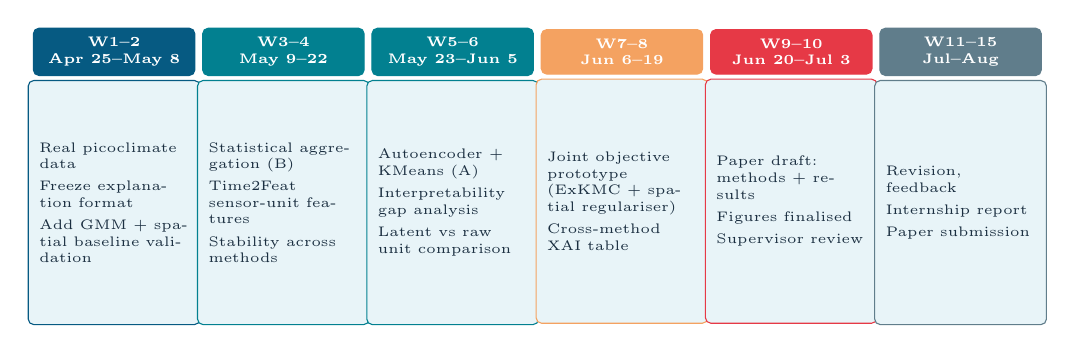
\begin{tikzpicture}
  \node[draw=cmid,fill=cmid,text=white,rounded corners=2pt,
    minimum width=2.05cm,minimum height=0.5cm,
    font=\bfseries\tiny,align=center] (h1) at (0,0) {W1--2\\Apr 25--May 8};
  \node[draw=cbg2,fill=cbg2,text=white,rounded corners=2pt,
    minimum width=2.05cm,minimum height=0.5cm,
    font=\bfseries\tiny,align=center] (h2) at (2.15,0) {W3--4\\May 9--22};
  \node[draw=cbg2,fill=cbg2,text=white,rounded corners=2pt,
    minimum width=2.05cm,minimum height=0.5cm,
    font=\bfseries\tiny,align=center] (h3) at (4.3,0) {W5--6\\May 23--Jun 5};
  \node[draw=cwarn,fill=cwarn,text=white,rounded corners=2pt,
    minimum width=2.05cm,minimum height=0.5cm,
    font=\bfseries\tiny,align=center] (h4) at (6.45,0) {W7--8\\Jun 6--19};
  \node[draw=cgap,fill=cgap,text=white,rounded corners=2pt,
    minimum width=2.05cm,minimum height=0.5cm,
    font=\bfseries\tiny,align=center] (h5) at (8.6,0) {W9--10\\Jun 20--Jul 3};
  \node[draw=cmuted,fill=cmuted,text=white,rounded corners=2pt,
    minimum width=2.05cm,minimum height=0.5cm,
    font=\bfseries\tiny,align=center] (h6) at (10.75,0) {W11--15\\Jul--Aug};
  \node[draw=cmid,fill=clight,text=ctext,rounded corners=2pt,
    minimum width=2.05cm,minimum height=3.1cm,
    font=\tiny,align=left,inner sep=4pt,text width=1.9cm,below=0.05cm of h1]{Real picoclimate data\\[2pt]Freeze explanation format\\[2pt]Add GMM + spatial baseline validation};
  \node[draw=cbg2,fill=clight,text=ctext,rounded corners=2pt,
    minimum width=2.05cm,minimum height=3.1cm,
    font=\tiny,align=left,inner sep=4pt,text width=1.9cm,below=0.05cm of h2]{Statistical aggregation (B)\\[2pt]Time2Feat sensor-unit features\\[2pt]Stability across methods};
  \node[draw=cbg2,fill=clight,text=ctext,rounded corners=2pt,
    minimum width=2.05cm,minimum height=3.1cm,
    font=\tiny,align=left,inner sep=4pt,text width=1.9cm,below=0.05cm of h3]{Autoencoder + KMeans (A)\\[2pt]Interpretability gap analysis\\[2pt]Latent vs raw unit comparison};
  \node[draw=cwarn,fill=clight,text=ctext,rounded corners=2pt,
    minimum width=2.05cm,minimum height=3.1cm,
    font=\tiny,align=left,inner sep=4pt,text width=1.9cm,below=0.05cm of h4]{Joint objective prototype\\(ExKMC + spatial regulariser)\\[2pt]Cross-method XAI table};
  \node[draw=cgap,fill=clight,text=ctext,rounded corners=2pt,
    minimum width=2.05cm,minimum height=3.1cm,
    font=\tiny,align=left,inner sep=4pt,text width=1.9cm,below=0.05cm of h5]{Paper draft:\\methods + results\\[2pt]Figures finalised\\[2pt]Supervisor review};
  \node[draw=cmuted,fill=clight,text=ctext,rounded corners=2pt,
    minimum width=2.05cm,minimum height=3.1cm,
    font=\tiny,align=left,inner sep=4pt,text width=1.9cm,below=0.05cm of h6]{Revision,\\feedback\\[2pt]Internship report\\[2pt]Paper submission};
\end{tikzpicture}
\vspace{3pt}
% \centering{\itshape\scriptsize\color{cmuted}$\sim$15 weeks remaining\\$\cdot$ 1--2 manuscripts target}
\end{frame}

% ── SLIDE 11 ────────────────────────────────────────────────────────────────
\begin{frame}{Scope Reminder}
\begin{block}{Current data status}
  The real PICOPATT data is still unavailable for the current context. The picoclimate work in the repository is a simulated test fixture used for validation only.
\end{block}
\vspace{0.5em}
\begin{itemize}
  \item Simulated picoclimate fixture: 4 timesteps, about 23 variables, used to test the pipeline structure.
  \item Real PICOPATT validation remains future work once the real data is available.
  \item Current focus: keep the explanation format stable and broaden the benchmark matrix.
\end{itemize}
\end{frame}

% ── SLIDE 12 ────────────────────────────────────────────────────────────────
\begin{frame}{What Changed Recently}
\begin{columns}[T,onlytextwidth]
  \column{0.52\textwidth}
  \begin{block}{Validated in code}
    \begin{itemize}
      \item Shapelet notebooks renamed and aligned under \texttt{shapelets\_}
      \item Cross-dataset stability run completed with 6 seeds
      \item HDBSCAN added to the picoclimate benchmark script
      \item Autoencoder + KMeans baseline already available and runnable
    \end{itemize}
  \end{block}

  \column{0.45\textwidth}
  \begin{block}{Governance update}
    \begin{itemize}
      \item Explanation output format is now treated as a contract
      \item Future methods must emit the same cluster-summary structure
      \item The goal is sensor-readable explanations, not feature-index-only narratives
    \end{itemize}
  \end{block}
\end{columns}
\end{frame}

% ── SLIDE 13 ────────────────────────────────────────────────────────────────
\begin{frame}{Evidence: Stability Across Datasets}
\begin{columns}[T,onlytextwidth]
  \column{0.58\textwidth}
  \centering
  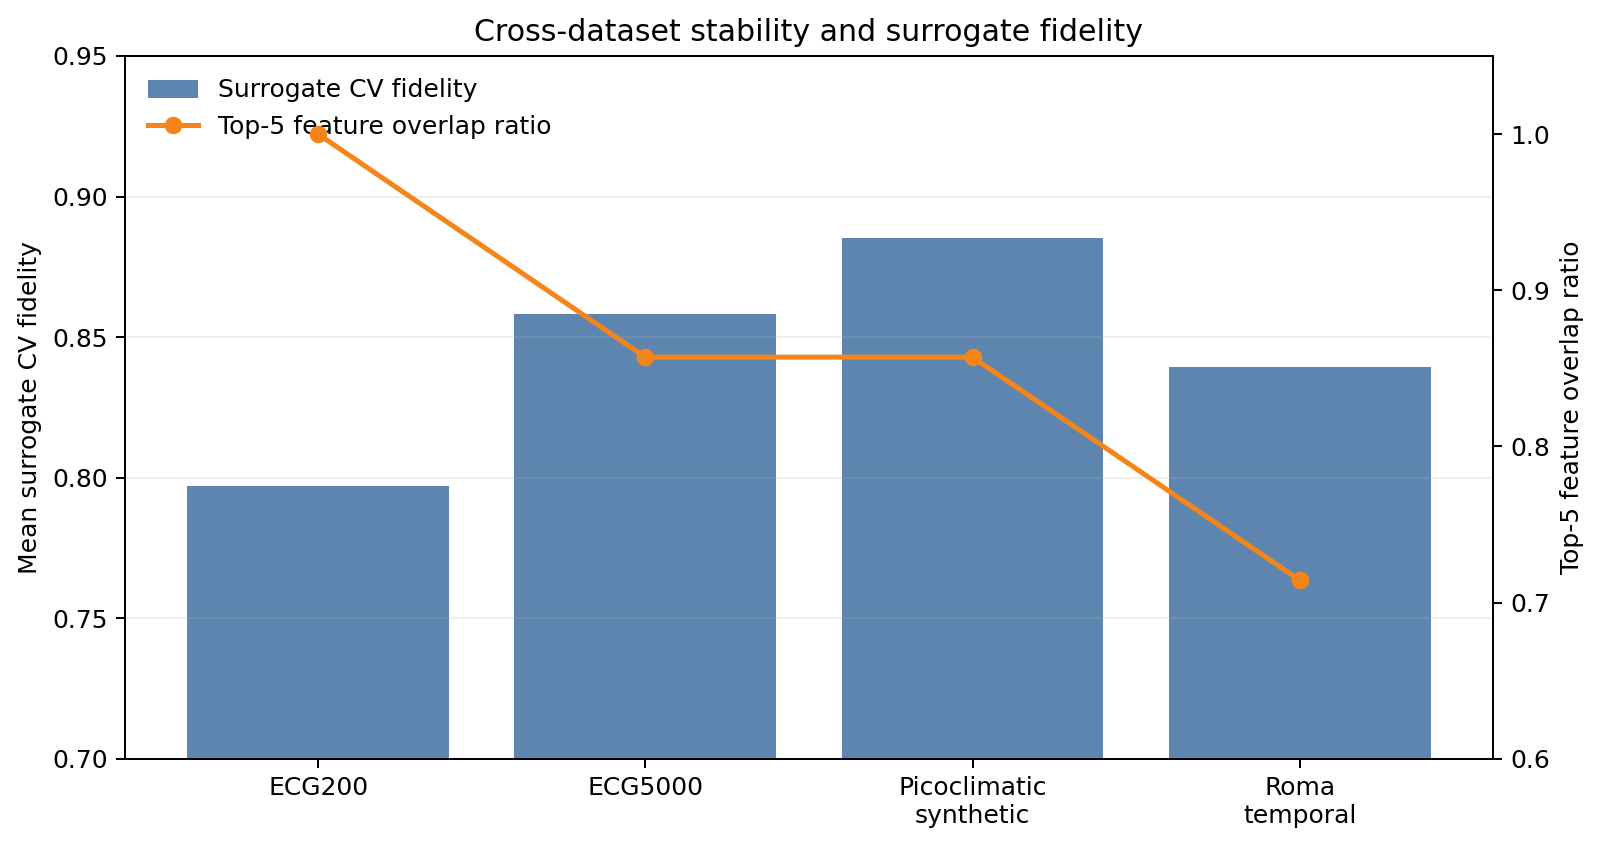
\includegraphics[width=0.96\linewidth]{figures/stability_summary.png}
  \column{0.38\textwidth}
  \begin{block}{What this slide should show}
    \begin{itemize}
      \item Surrogate CV fidelity band
      \item Top-5 SHAP overlap across 6 seeds
      \item The main robustness evidence
    \end{itemize}
  \end{block}
\end{columns}
\vspace{0.4em}
\begin{itemize}
  \item Reserve this space for the stability summary figure when you want the slide to show the actual chart.
\end{itemize}
\end{frame}

% ── SLIDE 14 ────────────────────────────────────────────────────────────────
\begin{frame}{Evidence: Deep Representation Baseline}
\begin{columns}[T,onlytextwidth]
  \column{0.58\textwidth}
  \centering
  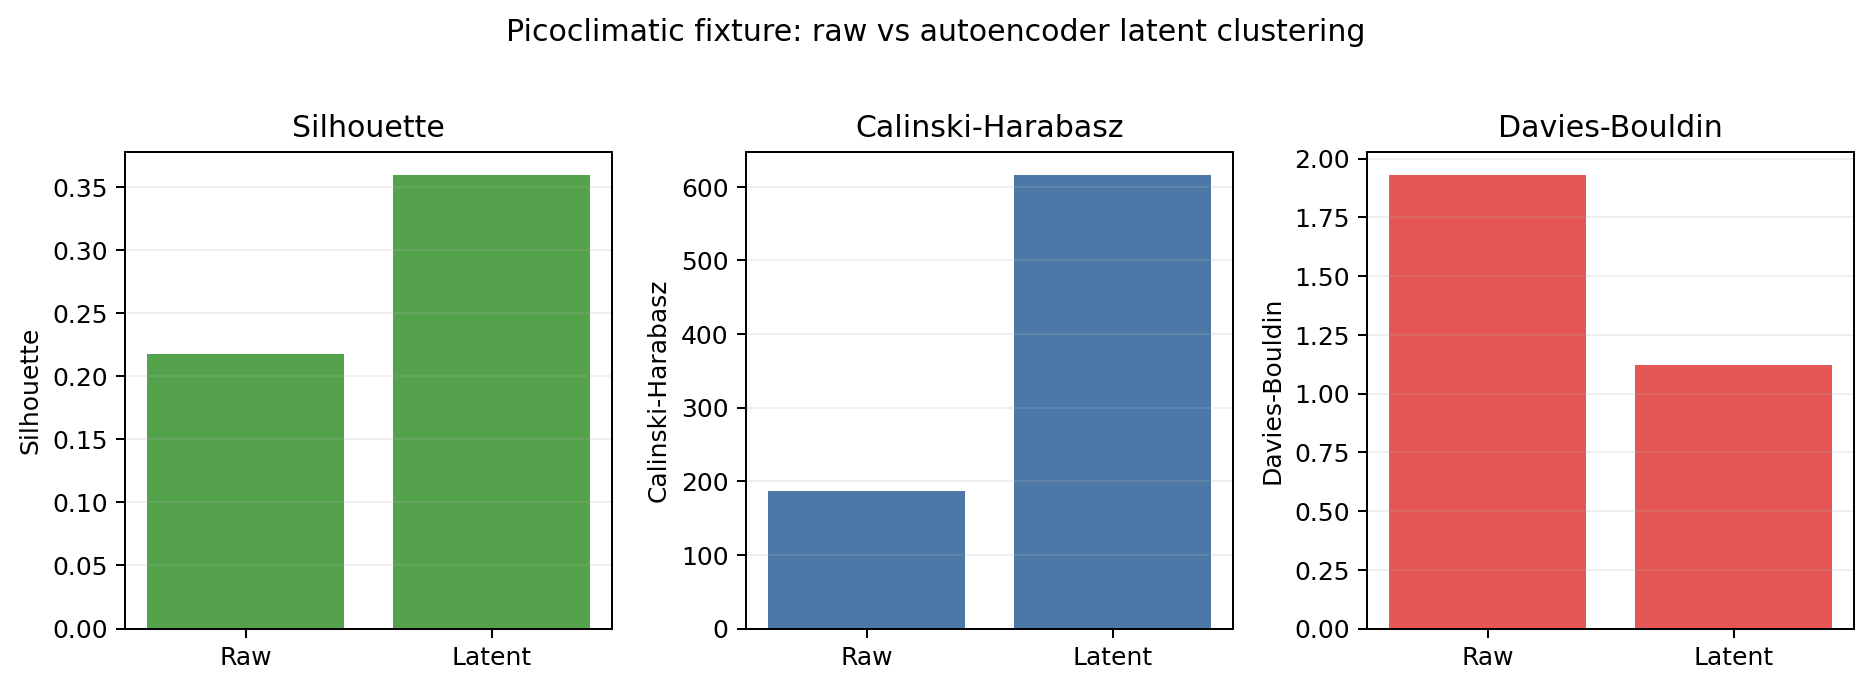
\includegraphics[width=0.96\linewidth]{figures/deep_representation_comparison.png}
  \column{0.38\textwidth}
  \begin{block}{Interpretation}
    \begin{itemize}
      \item Autoencoder baseline is the deep comparator
      \item Latent space improves clustering in the quick test
      \item Useful for the interpretability-gap story
    \end{itemize}
  \end{block}
\end{columns}
\end{frame}

% ── SLIDE 15 ────────────────────────────────────────────────────────────────
\begin{frame}{Evidence: Spatial Baseline Expansion}
\begin{columns}[T,onlytextwidth]
  \column{0.58\textwidth}
  \centering
  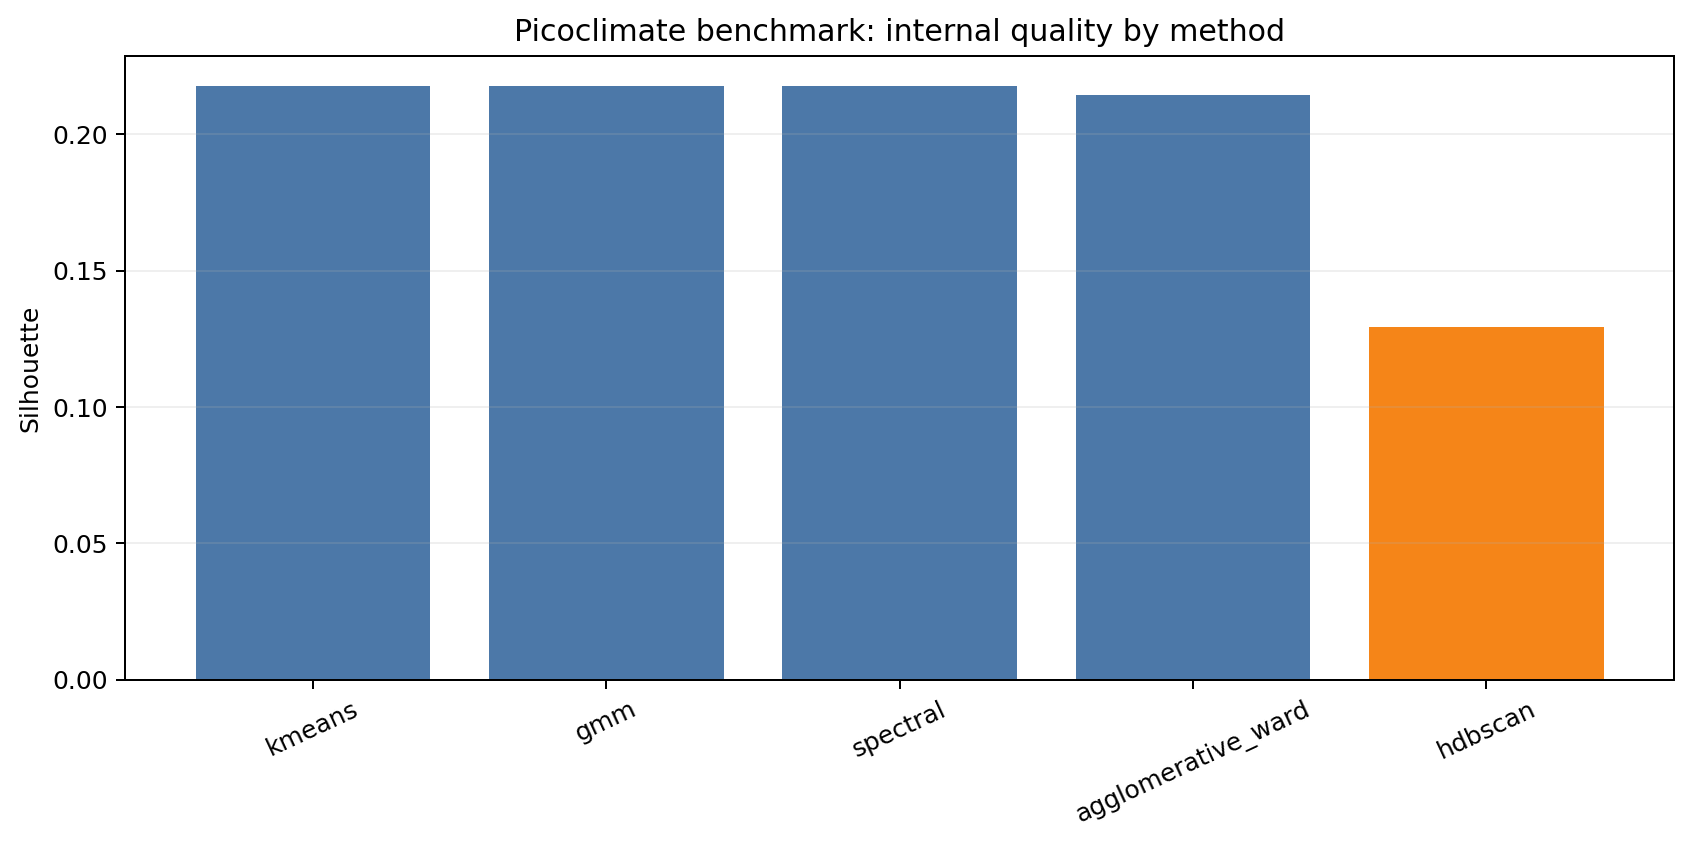
\includegraphics[width=0.96\linewidth]{figures/benchmark_silhouette.png}
  \column{0.38\textwidth}
  \begin{block}{Interpretation}
    \begin{itemize}
      \item HDBSCAN broadens the baseline set beyond KMeans / ExKMC
      \item Spatial density is now part of the benchmarking story
      \item Final PICOPATT benchmark still pending real data
    \end{itemize}
  \end{block}
\end{columns}
\end{frame}

% ── SLIDE 16 ────────────────────────────────────────────────────────────────
\begin{frame}{Interpretation Layer}
\begin{columns}[T,onlytextwidth]
  \column{0.48\textwidth}
  \begin{block}{What is already supported}
    \begin{itemize}
      \item Surrogate fidelity is high enough to defend model-faithful explanations.
      \item SHAP concentration already gives a compact narrative for the shapelet baseline.
      \item Stability is now measured rather than assumed.
    \end{itemize}
  \end{block}

  \column{0.48\textwidth}
  \begin{block}{What is still missing}
    \begin{itemize}
      \item Sensor-unit explanation template frozen across methods
      \item Spatial density comparators on real PICOPATT data
      \item A fuller joint-optimization method if the paper goes beyond a pipeline story
    \end{itemize}
  \end{block}
\end{columns}
\end{frame}

% ── SLIDE 17 ────────────────────────────────────────────────────────────────
\begin{frame}{Recommended Next Phase}
\begin{enumerate}
  \item Freeze the explanation output format and make every method emit the same cluster-summary schema.
  \item Keep ExKMC as the main interpretable clustering baseline for now.
  \item Extend the benchmark matrix with spatial methods; HDBSCAN is the first one now in place.
  \item Treat the autoencoder + KMeans path as the deep representation baseline.
  \item If the research contribution shifts toward methods, prototype the simplified ExKMC-style spatial regularizer next.
\end{enumerate}

\vspace{0.4em}
\begin{block}{Practical takeaway}
  The current repository is now ready for a Phase 2 story: simulated validation, stable explanations, and broader clustering baselines before moving to real PICOPATT data.
\end{block}
\end{frame}

% ── SLIDE 18 ────────────────────────────────────────────────────────────────
\begin{frame}{Reserved Figure Space}
\begin{block}{Future visuals}
  \vspace{0.8em}
  \centering
  \figureplaceholder{0.82\linewidth}{2.2cm}
\end{block}

\vspace{0.6em}
\footnotesize Suggested future figures: cluster profile heatmap, station map, sensor-unit explanation example, and a side-by-side comparison of stable vs unstable narratives.
\end{frame}

\end{document}
